% This is "www2010-sample.tex" copied from "www2005-sample.tex" V1.2 January 26 2004
% This file should be compiled with V1.4 of "www2010-submission.class"
%
% This example file demonstrates the use of the 'www2010-submission.cls'
% V1.4 LaTeX2e document class file. It is for those submitting
% articles to the WWW'04 Conference WHO DO NOT WISH TO 
% STRICTLY ADHERE TO THE SIGS (PUBS-BOARD-ENDORSED) STYLE.
% The 'www2010-submission.cls' file will produce a similar-looking,
% albeit, 'tighter' paper resulting in, invariably, fewer pages.
%
% ----------------------------------------------------------------------------------------------------------------
% This .tex file (and associated .cls V1.4) produces:
%       1) NO Permission Statement
%       2) WWW'04-specific conference (location) information
%       3) The Copyright Line with ACM data
%       4) NO page numbers
%
% ---------------------------------------------------------------------------------------------------------------
% This .tex source is an example which *does* use
% the .bib file (from which the .bbl file % is produced).
% REMEMBER HOWEVER: After having produced the .bbl file,
% and prior to final submission, you *NEED* to 'insert'
% your .bbl file into your source .tex file so as to provide
% ONE 'self-contained' source file.
%
% ================= IF YOU HAVE QUESTIONS =======================
% Questions regarding the SIGS styles, SIGS policies and
% procedures, Conferences etc. should be sent to
% Julie Goetz (goetz@acm.org) or Adrienne Griscti (griscti@acm.org)
%
% Technical questions only to
% Gerald Murray (murray@acm.org)
% ===============================================================
%
% For tracking purposes - this is V1.2 - January 26 2004
\documentclass{www2010-submission}
\usepackage{fancyvrb}

\begin{document}
%
\title{QueryMed: An Intuitive SPARQL Query Builder for Biomedical RDF Data}
%\subtitle{[Extended Abstract]
%\titlenote{A full version of this paper is available as
%\textit{Author's Guide to Preparing ACM SIG Proceedings Using
%\LaTeX$2_\epsilon$\ and BibTeX} at
%\texttt{www.acm.org/eaddress.htm}}}
%
% You need the command \numberofauthors to handle the "boxing"
% and alignment of the authors under the title, and to add
% a section for authors number 4 through n.
%
% Up to the first three authors are aligned under the title;
% use the \alignauthor commands below to handle those names
% and affiliations. Add names, affiliations, addresses for
% additional authors as the argument to \additionalauthors;
% these will be set for you without further effort on your
% part as the last section in the body of your article BEFORE
% References or any Appendices.

\numberofauthors{2}
%
% Put no more than the first THREE authors in the \author command

% NOTE: All authors should be on the first page. For instructions
% for more than 3 authors, see:
% http://www.acm.org/sigs/pubs/proceed/sigfaq.htm#a18

\author{
%
% The command \alignauthor (no curly braces needed) should
% precede each author name, affiliation/snail-mail address and
% e-mail address. Additionally, tag each line of
% affiliation/address with \affaddr, and tag the
%% e-mail address with \email.
\alignauthor Oshani Seneviratne\\
       \affaddr{Massachusetts Institute of Technology}\\
       \affaddr{Cambridge, MA}\\
       \affaddr{USA}\\
       \email{oshani@csail.mit.edu}
\alignauthor Rachel Sealfon\\
       \affaddr{Massachusetts Institute of Technology}\\
       \affaddr{Cambridge, MA}\\
       \affaddr{USA}\\
       \email{rsealfon@csail.mit.edu}
}
\date{15 Feb 2010}

\maketitle
\begin{abstract}
We have developed an open-source SPARQL query builder and result set visualizer for biomedical data, QueryMed, that allows end users to easily construct and run translational medicine queries across multiple data sources. 
\smallskip

QueryMed allows a flexible range of queries relevant to a wide range of biomedical topics and runs queries across multiple SPARQL endpoints.  The system is accessible for users who are unfamiliar with the SPARQL query language or the structure of the underlying ontologies. The system allows users to select the data sources that they wish to use, drawing on their specialized domain knowledge to decide the most appropriate data sources to query.  Users can add additional data sources if they are interested in querying endpoints that are not in the default list. The system automatically translates the user input into a SPARQL query for each individual endpoint, combines the results, and returns them to the user. After retrieval of the initial result set, query results can be improved  by iteratively modifying the original query terms, and by filtering the result list.  The advanced query functionality of the system allows the user to easily construct complex logical SPARQL queries that exploit the underlying structure of the RDF data. 
\end{abstract}

\keywords{Biomedical Ontologies, SPARQL, Query Federation, Query Building, Semantic Web, User Interfaces}

\label{system}

\section{QueryMed Overview}

\smallskip

\subsection{QueryMed Overview}


A general overview of QueryMed architecture is shown in Figure \ref{fig:architecture_detail.jpg}. The main components of the system are the user interface and the proxy server that takes input from the user and retrieves relevant biomedical data from remote SPARQL endpoints.   After a user submits a query from the user interface, the query is translated by the proxy server into individual SPARQL queries for each remote endpoint.  The query results are returned from the remote endpoints, combined by the proxy server, and presented to the user.   


%The system relies on two external resources: 

%\begin{enumerate}
%\item \textbf{SPARQL endpoints} that expose biomedical data.
%\item \textbf{Sources List} that gives a list of endpoints available to the user. This list is stored on the proxy server, but can be replaced by the user. 
%\end{enumerate}

\subsubsection{User Interface}

The QueryMed user interface is designed to be intuitive for the end user, yet flexible enough to permit a broad range of interesting queries.  The basic query interface allows the user to run simple queries, and is designed for maximal ease of use (Figure \ref{fig:initial_ui}).  The advanced search capabilities allow the user to easily construct complex logical queries that take advantage of the underlying structure of the biomedical ontologies.  The user interface also allows the user to iteratively refine queries, and displays the query results, which have been retrieved from multiple SPARQL endpoints.

\begin{figure}
\centering
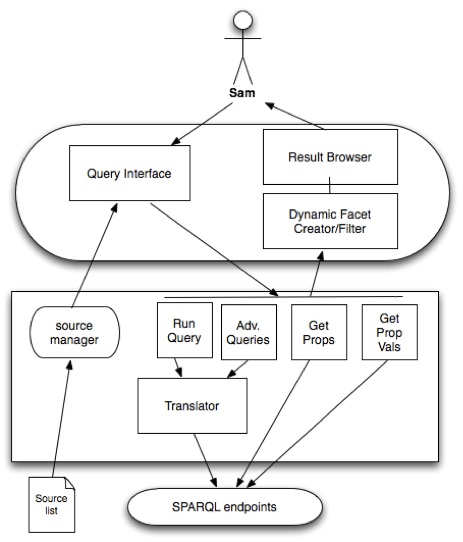
\epsfig{file=images/architecture_detail.jpg}
\caption{QueryMed Architecture}
\label{fig:arch_details}
\end{figure}

\smallskip


\begin{figure}
\centering
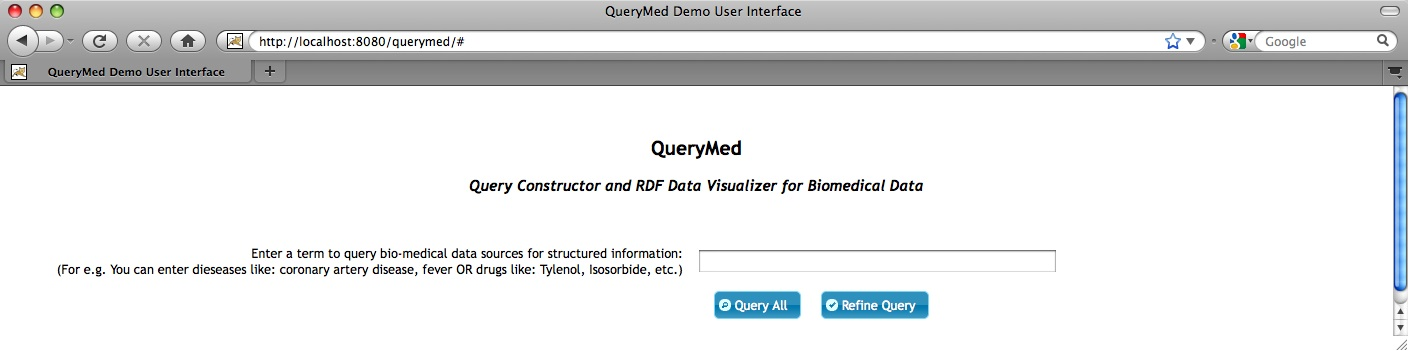
\epsfig{file=images/new_front.jpg,  width=3in}
\caption{Initial Basic Query Interface}
\label{fig:initial_ui}
\end{figure}

\smallskip

\begin{table*}
\begin{center}
\begin{tabular}{| p{1.8cm} | p{2cm} | p{1.8cm} | p{1.8cm}| p{1.8cm}| p{1.8cm}| p{1.8cm}| p{1.8cm} |}
\hline
 & \textbf{Hybrid Interface (Combines Querying \& Browsing)} & \textbf{Provides Local Caching} & \textbf{Queries Multiple Sources} & \textbf{Dynamic Addition of Sources} & \textbf{Allows Keyword Queries} & \textbf{Open Source} & \textbf{GUI} \\
\hline
\textbf{QueryMed}  & Yes & Yes & Yes & Yes & Yes & Yes & Yes  \\
\hline
\textbf{SMART}  & No & Yes & Yes & No & No & Yes & Yes  \\
\hline
\textbf{DARQ}  & No &  No & Yes & N/A & No & Yes & No  \\
\hline
\textbf{GoWeb}   & Yes & No  & Yes & No & Yes & No & Yes  \\
\hline
\textbf{BioGateway}   & Yes & Yes & Yes & No & No & Yes & Yes  \\
\hline
\textbf{Twinkle}   & No & No & Yes & No & No & Yes & Yes  \\
\hline
\end{tabular}
\caption{Comparison of selected features of the QueryMed system with other related systems.}
\label{comparison}
\end{center}
\end{table*}

\subsubsection{Proxy Server}

The proxy server acts as an intermediary between the user interface and the remote SPARQL endpoints.  Its functionality is twofold: 


\begin{enumerate}
\item Execute the SPARQL queries at the relevant remote SPARQL endpoints and consolidate the results to be presented in the user interface.
\item Cache the results of the current query so that refinements of the query will have reduced network and query execution latency.
\end{enumerate}


The specific components in the Proxy Server are as follows.

\begin{itemize}

\item \textbf{Source Manager:} The Source Manager reads the source list and populates the default query list on the user interface. It also keeps track of the default endpoints, the currently selected endpoints, and the endpoints that have been dynamically added.

\item \textbf{Translator:} The Translator is responsible for translating the user query into valid SPARQL syntax.  The Translator obtains the parameters to construct the query from the input the user specifies in the Query Interface, and dynamically constructs a SPARQL query based on the user input.
% The user has to specify the data source(s) to query, and can give specific values for one or many of the properties available for the data available to restrict the query space. 



\end{itemize}

\subsubsection{Implementation}

QueryMed is implemented in Java in the backend and JavaScript, HTML and CSS in the frontend.  In the backend, the Jena library \cite{McBride} is used to run the SPARQL queries and 4-store~\cite{4store} is used as a triple store to provide caching support.  The JQuery library \cite{Resig} was used to develop an attractive user interface.   

%\subsection{A Sample Use Case}

%A physician is interested in finding semantic web resources related to coronary artery disease.  She first tries a basic search over all default resources, by entering ``coronary artery disease" in the input search box.   She then sees a list of disease names in the Diseasome database and drugs in DailyMed and Drugbank that relate to coronary artery disease displayed in a table.  She can then filter the results using additional search terms.  For example, she knows that the route of administration of the drug that she is looking for is injection, so she filters the drug query results on the route of administration field using the query term ``injection."  She then prints the table of results.

%She is now interested in finding relevant clinical trials for her patient.  However, the clinical trial database LinkedCt is not in the default set of endpoints, so she selects the ``Refine Query" option to choose additional endpoints to search.  She sees a list of default endpoints, and selects the ``Add" option to include an additional endpoint.  After entering the name and URL of the LinkedCT endpoint, she is able to search for clinical trials for which her patient may be eligible.  

%She is also interested in further refining her search.  She uses the advanced search option to construct a boolean query that takes advantage of the underlying structure of the RDF data in the database.  She searches diseasome for a list of diseases whose class is ``Cardiovascular" or for which the associated gene is ``ABCA1."  Using the QueryMed advanced search interface, the complex SPARQL query corresponding to her question is automatically constructed, and she can view the query results conveniently displayed in a table.


\subsection{QueryMed Resources}

The source code for the Querymed system is available at the QueryMed Google Code project: \\
http://code.google.com/p/querymed

\smallskip

A video illustrating a sample use case can be found at: \\
http://dig.csail.mit.edu/2010/Papers/www-ws-colab-science/\\
videos



\section{Related Work}
\label{related}

A number of existing tools aim to provide a user-friendly interface for browsing semantic web data, or to allow users to perform federated queries. 

Table \ref{comparison} compares selected features of the QueryMed system with other related systems. The QueryMed system was unique among the systems that we found in that it allows endpoints to be dynamically added by the user, and provides a hybrid interface that enables the users to both query and browse data.  Other features of the QueryMed system that distinguish it from similar systems include the ability both to perform keyword queries and to construct more advanced queries taking advantage of the structure of the data.  This feature increases the ease of use of our system relative to other similar systems.  Furthermore, the Javascript-based user interface of the QueryMed system, implemented using the JQuery library, makes our user interface particularly attractive, easy to interact with, and capable of handling a variety of user input events.  Another unique feature of our system is the property-based advanced query interface. This interface enables users to take advantage of the structure of the underlying ontologies used to represent the data without prior knowledge of the ontology structures. 

\section{Conclusion}
\label{conclusion}

The main contributions of our system are: dynamic construction of complex SPARQL queries based on intuitive user input; dynamic addition of user-specified endpoints; and ability to run queries over multiple endpoints. Because our system is flexible and easy to use, we believe it will be of use to the biomedical community.  We also believe that developing systems such as such as QueryMed, which make SPARQL endpoints  easily accessible to end users, will entice more people to expose their data as linked open data.

%\section{Acknowledgments}

\bibliographystyle{abbrv}
\bibliography{references}  

\end{document}
